\begin{center}
    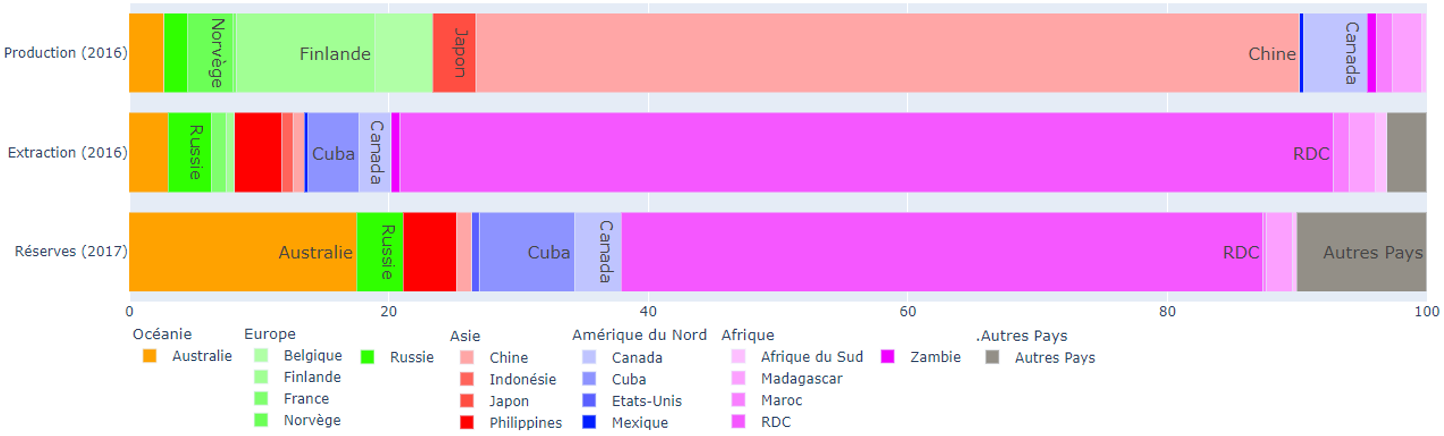
\includegraphics[width=\textwidth]{Illustration métaux/Cobalt.png}
\end{center}

\begin{center}
    \textbf{Usages et consommation}
\end{center}
La fabrication de batterie (véhicules électriques et électroniques) utilise 58\% de la production mondiale de cobalt. Le deuxième usage de cobalt est la fabrication de superalliages avec 15\%.
\begin{center}
    \textbf{Prospective}
\end{center}
\begin{multicols}{2}
    \begin{center}
        \textit{Total cobalt demand by sector and scenario}
    \end{center}
    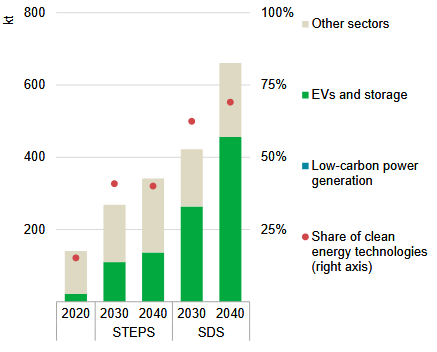
\includegraphics[width=0.45\textwidth]{Illustration métaux/Cobalt prospective.png}
    \vfill\null
    \columnbreak
    La décarbonation des activités humaines va impliquer une forte hausse de la demande en cobalt pour la fabrication des véhicules. Le taux de croissance annuel moyen de la production de cobalt raffiné a été de 7,4\% entre 2009 et 2019. 
    L'évolution de la demande en cobalt est très dépendante des choix technologiques pour les batteries suivis. 
    La chaîne d'approvisionnement en cobalt est amenée à rester concentré en Chine et en République démocratique du Congo.
    
    
\end{multicols}
\begin{center}
    \textbf{Production et recyclage}
\end{center}
Le cobalt est un métal avec une très forte concentration économique pour la production brut avec la République Démocratique du Congo et raffinée avec la Chine. Par ailleurs, la Chine influe sur de nombreux actifs de RDC \textit{via} des investissements. Le taux de recyclage du cobalt est d'environ 35\%. La production minière dépasse les 120 kt/an.
\begin{center}
    \textbf{Substituabilité}
\end{center}
Dans la fabrication des batteries, le cobalt est substituable par un changement de technologie ou par des changements de compositions chimiques.
\begin{center}
    \textbf{Prix}
\end{center}
Le prix du cobalt est volatile. Le prix moyen est de 31 176 US\$/t en 2020. Avec une valeur du marché dépassant les 4.3 G US\$.
\clearpage
\begin{center}
    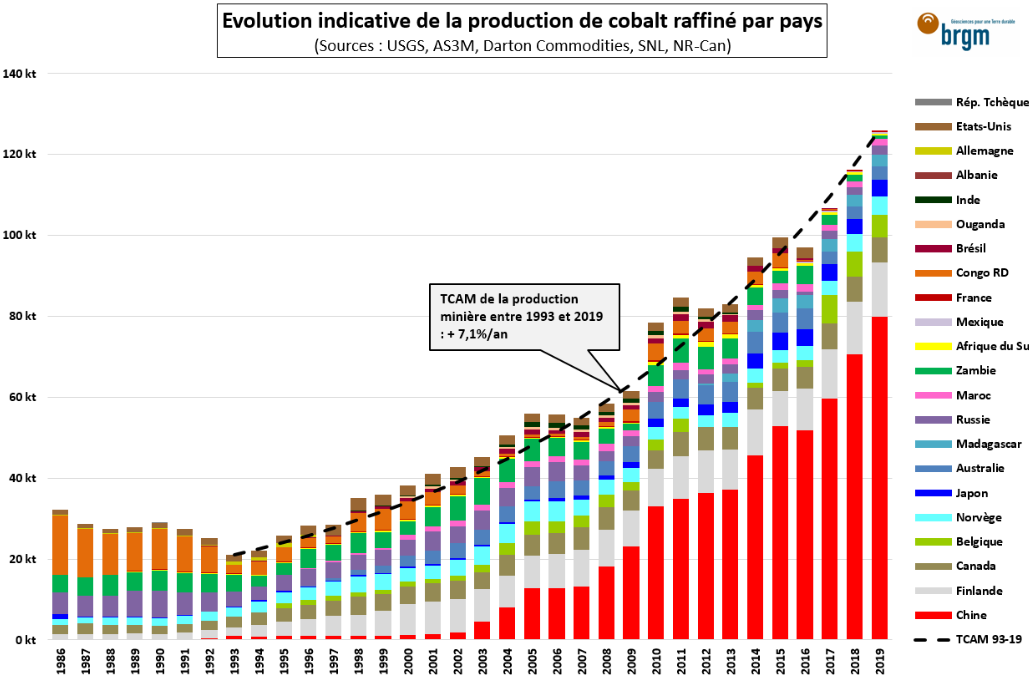
\includegraphics[width=12cm]{Illustration métaux/dynamique_cobalt.png}
\end{center}
\begin{center}
    \textbf{Evènements géopolitiques}
\end{center}
Des perturbations d'approvisionnement locales ont été recensées. En 2015, le site de production de Chambishi a été perturbé par des tension avec la RDC, entraînant des suspensions dans l'approvisionnement par ce site. En 2007, des différends politiques ont perturbé l'approvisionnement en cobalt par la RDC pendant près d'un an entrainant des augmentations de prix. (\cite{hatayama_adopting_2018})

\begin{multicols}{2}
    \begin{center}
      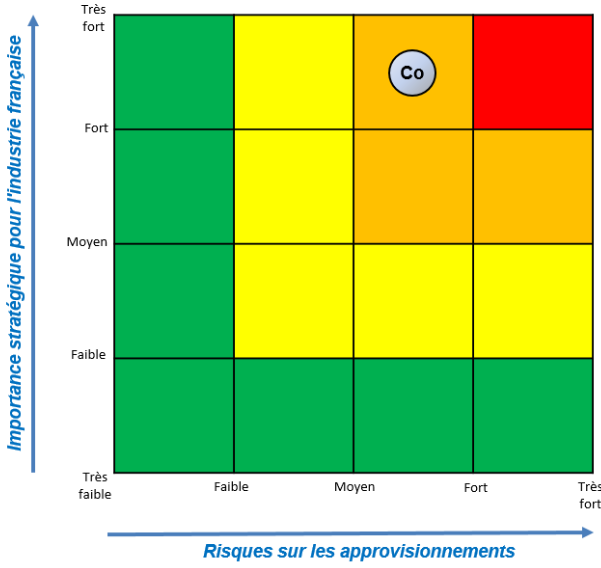
\includegraphics[width=0.35\textwidth]{Illustration métaux/Cobalt_criticité.png} 
    \end{center}
    \begin{center}
    \textbf{Criticité en France}
    \end{center}
    Le cobalt est particulièrement important pour l'industrie du fait des nombreux secteurs d'usages comme l'énergie, l'aéronautique, la défense et l'autombile. La forte concentration du marché engendre un risque sur l'approvisionnement important.
\end{multicols}

\begin{center}
    \textbf{Risques spécifiques}
\end{center}
Une part significative de la production minière de cobalt est issue de petites mines artisanales, bien que ces mines permettent de stabiliser les prix de marché grâce à leur production flexible. La fiabilité de l'approvisionnement par ces mines est affaiblie par les vulnérabilités sociales et économiques de ces sites de production. Ces petites mines artisanales sont particulièrement peu régulées incluant des conditions de travail dangereuses et la présence de travail des enfants.\\
Le cobalt est souvent un sous-produit du cuivre et du nickel. En conséquence, il est possible qu'il n'y ait pas d'investissements dans la production de cobalt tant que le marché du cuivre et du nickel n'envoient pas de signaux pour investir dans la production.